\chapter{Enhancing Visual Features}
\label{chapter:VisFeatChapter}

Finding good feature vector representations for the input images and videos is a
very important task for successful design of a captioning system.
%%
Such a feature representation should be compact, but also able to encode all the
information relevant for the task. 
%%
For the image captioning task, the feature vector should capture all the objects in
the image, their most essential properties such as color, their absolute
position and relative location to each other, along with the type of the scene
these objects are located in.
%%
In case of video captioning, apart from all the above mentioned information, the
feature vector should also encode sufficient temporal information to enable
recognizing actions, order of events, etc.

In this chapter, we will study different visual features for both images and
videos in order to improve the performance of the captioning system over the
baseline presented in Chapter~\ref{chapter:baseline}.
%%
The chapter is divided into two main sections, with one discussing the visual
features used to represent images and the other describing the features used to
encode videos.

%%===========================================================================%%
\section{Image Feature Extraction}
\label{sec:ImageFeat}

Activation values extracted from the deep Convolutional Neural Network (CNN)
layers are the primary features used to represent images in the captioning
models presented in this thesis.
%%
The CNN features are able to encode a rich variety of information, including
scene context, object type, etc.\@, as seen from its performance in the baseline
model.
%%
However, this representation is still very dense and probably (as seen later in
experiments) inefficient for the language model to be able to extract the
information it needs to generate correct captions.
%%
It is also unclear to what extent these features encode multiple objects and
object locations, since they are trained on the ImageNet task involving
recognizing a single object class.

Thus, in a bid to improve the performance over the baseline model, language
model is provided with additional features which explicitly encode presence
of objects, scene types and object location.
%%
To achieve this, explicit object detectors and scene detectors are trained based
on the CNN features.
%%
Additionally, features encoding object localization are constructed based on
outputs from Faster Region-based Convolutional Neural Network
(R-CNN)~\cite{ren15fasterrcnn}.
%%
In the following subsections we will discuss the exact details of the processes
used to extract all of the above features from input images. 
%%----------------------------------%%
\subsection{Convolutional Neural Networks}
%%----------------------------------%%
Convolutional Neural Networks have in the recent years become the most widely
used models for practically all tasks related to image classification and
understanding.
%%
It is shown in~\cite{Donahue2014} and~\cite{Razavian2014CVPR} that activations
of the fully-connected layers of a CNN trained for image classification task act
as a general feature representation of the image and can be successfully used to
solve other tasks as well.
%%
In line with this, image features are extracted here from different CNN
architectures pre-trained on two large datasets namely,
ImageNet~\cite{ImagenetOrig} and MIT Places~\cite{Zhou2014NIPS}, originally
aimed for object and scene classification, respectively.
%%

The CNNs used here are based on the widely used
GoogLeNet~\cite{DBLP:journals/corr/SzegedyLJSRAEVR14} and VGG~\cite{Simonyan14c}
architectures. 
%%
Both of these architectures achieved good results in the ILSVRC 2014 object
classification challenge, coming first and second, respectively, in the
competition.
%%
In this work, the GoogLeNet features are used both as a direct input to the
language model and to train the place and object detector modules, while the VGG
net features are only used for the latter.

\subsubsection{GoogLeNet} 
\label{subsec:gCNN}
The main idea behind the GoogLeNet~\cite{DBLP:journals/corr/SzegedyLJSRAEVR14}
architecture is to use small dense structures like $1\times1$, $3\times3$
convolutions to mimic a large sparse layer.
%%
For this purpose they utilize the \emph{Inception} modules consisting of
$1\times1$, $3\times3$ and $5\times5$ convolutions and maximum pooling layers.
%%
This network achieved the top-5 error rate of $6.67\%$ in the 1000 class ILSVRC
2014 Classification Challenge, finishing first in the competition.

We use two different versions of the GoogLeNet features in our experiments.
%%
Features from GoogLeNet trained on ImageNet~\cite{ImagenetOrig} dataset are used
as direct input to our language model (referred to as "\emph{gCNN}" in the rest
of the text), whereas features from the GoogLeNet trained on MIT
Places~\cite{Zhou2014NIPS} data (referred to as "\emph{pCNN}" in the rest of the
text) are used to construct scene recognition features which are used as
auxiliary inputs to our language model.
%%

To extract \emph{gCNN} features, we use the activations from the
\emph{5th Inception module}, having the dimensionality of 1024.
%%
We augment these features with the reverse spatial pyramid pooling proposed
in~\cite{Gong2014} with two scale levels.
%%
The first scale is just the full image rescaled to the size of $224\times224$.
%%
The second level consists of a $3\times3$ grid of overlapping patches of size
$128\times128$ with stride of 64, and horizontal flipping.
%%
The activations of these regions are then reduced to a single 1024 dimensional
feature vector by using average pooling or by just using the central crop.
%%
Finally, the activations of the two scales are concatenated resulting in
2048-dimensional features.
%%
Note that due to two different pooling methods on the second scale, we obtain
two somewhat different feature vectors of 2048 dimensions from the same network.
%%
Our final \emph{gCNN} feature vector of size 4096 dimensions is obtained by
concatenating these two feature vectors.
%%
This is also the feature vector used as the input to our baseline image
captioning model. 

The same procedure described above for the ImageNet trained GoogLeNet has
also been followed with the Places data trained GoogLeNet, with the exception
that instead of the Inception module, the \emph{3rd classification branch} has
been used as the activation layer where the feature vectors have been extracted.
%%
In this case, in addition to the mean and center pooling in the second scale of
reverse spatial pyramid, we also use maximum pooling, and thus obtain three
different features with the dimensionality of 2048 each.
%%
Note that the term \emph{pCNN} refers collectively to this set of three features.

\subsubsection{VGG network} 
VGG network was introduced in \cite{Simonyan14c}, where the authors study the
effect of depth on the performance of convolutional networks.
%%
The salient feature of this architecture is the exclusive use of small $3\times3$ and
$2\times2$ convolutional filters throughout the network.
%%
This helps in keeping the number of parameters small even with the increased depth.
%%
This network achieves the top-5 error rate of $7.3\%$ in the 1000 class ILSVRC
2014 Classification Challenge, finishing second in the competition.

Two variants of the VGG net, namely the 16- and 19-layered ones from
\cite{Simonyan14c}, are used in the experiments reported here.
%%
From both the variants, we extract the activations of the network on the second
fully-connected 4096-dimensional \emph{fc7} layer for the given input images
whose aspect ratio is distorted to a square.
%%
Ten regions, as suggested in~\cite{Krizhevsky2012}, are extracted from all
images and average pooling of the region-wise features are used to generate the
final features.
%%

\subsection{Object Detectors}
\label{subsec:svm80}
%%----------------------------------%%

As mentioned before, the CNN features are augmented with explicit object
detector features where each dimension represents the presence or absence of one
of the 80 object categories defined in the COCO dataset~\cite{Lin2014}.
%%
These 80 categories consists of common object types such as \emph{person},
\emph{car}, \emph{bus}, \emph{dog}, \emph{cat}, \emph{table}, \emph{chair},
\emph{pizza}, \emph{banana}, \emph{laptop}, etc.
%%

To construct the explicit object detector features, 80 separate SVM
classifiers~\cite{cortes1995support} are trained on the COCO 2014~\cite{Lin2014}
training set to detect each of these 80 object categories.
%%
Image features extracted using the previously described five CNN-based
ImageNet-trained VGG and GoogLeNet features are used as input to the 80 object
detector SVMs. 
%%
In particular, we here utilized linear SVMs with homogeneous kernel
maps~\cite{Vedaldi2010} of second order to approximate the intersection kernel.
%%
Furthermore, we used two rounds of hard negative mining~\cite{Li2013} and
sampled $5\,000$ negative examples on each round.

For each image we thus have 15 SVM outputs for each class (five features times
initial and two hard negative trained models) that we combine with simple
arithmetic mean in the late fusion stage.
%%
The 80 fused output values, one for each object category, are then concatenated
to form a class membership vector for each image.
%%
These vectors we optionally use as inputs to the LSTM network and we denote it
as ``\emph{SVM80}'' in the rest of the thesis.

\subsection{Scene Detectors}
%%----------------------------------%%
%%
\begin{figure*}[tbh] 
  \centering
  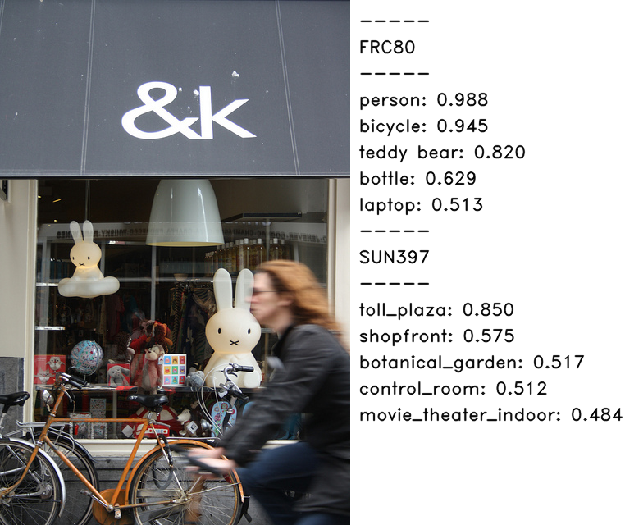
\includegraphics[width=0.6\textwidth]{./images/95474.pdf} 
  \caption{Visualization of top five detected objects~(FRC80) and scene
  types~(SUN397) along with the associated confidence scores for an image from
  the MS-COCO validation set.}
  \label{fig:COCODetVis} 
\end{figure*}

%\begin{figure}[t]
%    \begin{minipage}[c]{0.45\linewidth}
%        %\begin{center}
%            \includegraphics[width=\textwidth]{images/COCO_train2014_00000095474.jpg}
%        %\end{center}
%    \end{minipage}\hfill
%    \begin{minipage}[c]{0.52\linewidth}
%    \begin{tabular}{c|c|c|c|}
%          \cline{2-4}
%            \textbf{C1:} a beach with people relaxing on a \underline{sunny day}. \\
%            \textbf{C2}: people are relaxing on the beach where there is a \underline{big rock}. \\
%            \textbf{C3}: a beach with a group of people with surf boards and \underline{umberellas}. \\
%            \textbf{C4}: a group of people enjoy a beach near a lagoon filled with \underline{crystal blue
%            water}. \\
%            \textbf{C5}: a \underline{man walking} on a beach with his surf board in a case. \\
%    \end{minipage}
%  \vspace*{-3mm}
%  \caption{Visualization of top five detected objects~(FRC80) and scene
%  types~(SUN397) along with the associated confidence scores for an image from
%  the MS-COCO validation set.}
%  \label{fig:COCODetVis} 
%\end{figure}



In order to provide the language model with explicit information on the visual
environment or the scene type of the images, we used the SUN Scene
Categorization Benchmark database~\cite{Xiao2010} and~\cite{Xiao2014} to create
a bank of visual detectors specialized for scene recognition.
%%
The version of the database we used contains 108,756 images associated with one
of 397 scene categories.
%%
The 397 categories include three major classes --- namely indoor, outdoor-natural
and outdoor-man-made --- and common scene types including \emph{kitchen},
\emph{living-room}, \emph{shower}, \emph{tennis-court}, \emph{courtroom},
\emph{beach}, \emph{dock}, \emph{airfield}, \emph{dam} etc. 

We extracted both ImageNet data trained and MIT Places data trained GoogLeNet
CNN features, as described in the previous section, for the images in the SUN
database.
%%
We used features of all the images (not only the training split) for
training Radial Basis Function (RBF) Support Vector Machines (SVMs) with the
LIBSVM software~\cite{LIBSVM}.
%%
As we had three slightly different versions of each of the feature types, we
obtained the total of six SVM detectors for each scene category.

We applied each of the detectors to the images of the COCO dataset and used the
simple arithmetic mean for the late fusion of the detector outputs.
%%
The concatenation of the fused category-wise detector outputs results in
397-dimensional feature vectors for the respective images.
%%
These feature vectors are referred to as ``\emph{SUN397}'' in the rest of the
thesis.
%%
Figure~\ref{fig:COCODetVis} shows the top five detected scene categories using
the \emph{SUN397} features for an image from the COCO validation set.

%% --------------------------------------
\subsection{Spatial Map Encodings}
\label{sec:frcnnfeat}
%%----------------------------------%%
Another important source of information relevant to generating captions is the
relative location of the objects in the image. 
%%
Knowing the locations of the objects helps to infer their roles and actions in
the scene and also to choose the right adjectives to describe their positions.

For this purpose we use an object detector network, specifically the Faster
Region-based Convolutional Neural Network~(R-CNN) proposed in
\cite{ren15fasterrcnn}, to detect the multiple objects in the input image and to
predict their bounding boxes.
%%

We project the object bounding boxes onto a non-overlapping $m \times n$ grid
over the image.
%%
Each of the 80 object categories, $c$, maintains its own grid $F_c$.
%%
Each grid cell, $F_c(i,j)$, accumulates the intersection over union~(IoU) value
of any overlapping bounding box of that object category. 
%%
This IoU value is also scaled with detection confidence score generated by the
Faster R-CNN for that bounding box.
%%
Thus, we get 80 spatial maps of size $m\times n$. 
%%
These representations are then concatenated to produce an $m\times
n\times80$~-dimensional feature vector.
%%
The value of the feature vector component corresponding to the class $c$ and the
grid cell position $(i,j)$ can be computed as 
%%
\begin{equation} 
\label{eqn:Iou} 
F_c(i,j) = \sum_{b_k \in \text{\it BB}(c)}p(b_k)\frac{ A(b_k \cap G(i,j))}{A(b_k \cup G(i,j))} \;, 
\end{equation}
%%
where $A(\cdot)$ is the pixel area, $\text{\it BB}(c)$ are the bounding boxes
detected for objects of class $c$, $p(b_k)$ is the confidence assigned by the
detector to box $b_k$ and $G(i,j)$ is the grid cell at position $(i,j)$.
%%
We abbreviate these features as ``$m$$\times${}$n$IoU'' in the result tables.

We also experiment with replacing the bounding box with a Gaussian whose mean is
at the center of the bounding box and standard deviation is the length of the
box diagonal.
%%
Then, instead of the IoUs, each grid cell accumulates the integrals of the
Gaussians in their overlapping region as
%%
\begin{equation} \label{eqn:Gauss} F_c(i,j) = \sum_{b_k \in \text{\it
        BB}(c)} p(b_k)\text{\hspace*{-7mm}}\iint\displaylimits_%
{\text{\hspace{9mm}}b_k \cap G(i,j)}\text{\hspace*{-5mm}}
N(x,y,\text{center}(b_k),\text{diag}(b_k)) dx dy \; , \end{equation}
%%
\noindent where $BB(c)$ is the set containing bounding box object proposals for
category $c$, $p(b_k)$ is the confidence assigned by the detector to the
bounding box proposal $b_k$, $G(i,j)$ is the grid cell at position $(i,j)$ and
$N(x,y,\mu,\sigma)$ are Gaussians in $x$ and $y$ variables of given mean $\mu$
and standard deviation $\sigma$.
%%
The double integral in the above equation is done computed the area of intersection
between bounding box, $b_k$ and grid cell $G(i,j)$, $b_k \cap G(i,j)$.
%%
We abbreviate these features as ``$m$$\times${}$n$Gauss'' in the result tables.

As an alternative to the $m\times n$ non-overlapping grid, we have used also
``$m+n$ partitioning'' of the images.
%%
By this we mean that the images are split into $m$ horizontal and $n$ vertical
regions, each of equal width and equal height, respectively.
%%
The localization information provided by this representation is not as accurate
as that of the $m\times n$ grid model.
%%
Instead, it can be argued to be more robust against variations in the relative
placements of the objects.
%%
The calculation of these features is analogous to that of the grid-based ones,
only the definition of the grid cells $G(i,j)$ is different.
%%
We abbreviate these features as ``$m$+$n$Gauss'' in the figures and result
tables.

By setting the grid size parameters $m=n=1$ we lose all localization information
and get plain Faster R-CNN based object detector feature vectors, similar to the SVM80
features described in the previous section.
%%
These vectors are referred to as ``FRC80'' in the rest of this text. 
%%
An illustration of the top five objects detected using the \emph{FRC80} features
for an image from the COCO validation set is shown in
Figure~\ref{fig:COCODetVis}.

%%
We have to note here that it is computationally relatively expensive to extract
these features, as  running the Faster-RCNN network on the input image which,
despite the moniker, is still much slower than running a single CNN such as the
GoogLeNet on the input image.

%%===========================================================================%%
\section{Video Feature Extraction}
\label{sec:VideoFeat}
We use two different paradigms for video feature extraction.
%%
The first one is to treat the video as just a sequence of 2-D static images and
use CNNs trained on ImageNet~\cite{ImagenetOrig} to extract static image
features from these frames.
%%
The second approach is to treat the video as 3-D data, consisting of a
sequence of video segments, and use methods which also consider the variations
along the time dimension for feature extraction.
%%

In both the approaches above, pooling techniques are used to combine multiple
frame or segment level features into one video-level feature vector.
%%
Then number of feature vectors can also vary depending on the length of the
video.
%%
Since our language model cannot take arbitrary number of feature of vectors as
input, we need to further compress these multiple feature vectors into a single
video feature vector. 
%%
We use mean pooling, which is just taking the average of these feature vectors,
to reduce them to a single vector.

%%----------------------------------%%
\subsection{Keyframe and Multi-Frame Features}
In this subsection we will discuss the frame-level features used in the video
captioning model proposed in this thesis.
%%
The frame-level video features are extracted by treating the video as a bag of
static images, and applying the same feature extraction techniques used for
image captioning to these video frames.
%%
The key idea is to capture details of the scenes shown in the video, objects
present in it and their attributes.
%%
If the clip is very short and consists of only a single shot, then it might be
sufficient to extract these features from a single keyframe extracted from the
center of the video. 
%%
However, if the video clip is long, one will need to extract the frame-level
features from multiple frames, to sufficiently summarize the content in the
video.
%%

In order to keep the computational time reasonable, all the feature extraction
methods discussed before for images are not used on videos.
%%
Instead, only the gCNN features and the explicit object recognition
features~(\emph{SVM80}) are extracted from the video frames.
%%
Computational efficiency is also improved by sampling only the keyframe in case
of LSMDC dataset and one frame every second in MSR-VTT dataset for feature
extraction.
%%
The feature extraction procedure for both gCNN and SVM80 features remain the
same as described before for images in sections~\ref{subsec:gCNN} and
\ref{subsec:svm80}. 

%% ---------------------------------------------------------------------------
\subsection{Segment-Level Features}
%%----------------------------------%%
Although the frame-level features do well in capturing the overall scene
context of the videos, they fail to recognize actions and other motion-related
events.
%%
This is because lot of action in videos involve very local motion patterns,
which is hard to capture when looking at frames individually.
%%
Such actions can occur even without any whole objects moving, and thus causing
the CNN feature extractors to not notice hardly any change.
%%

The motion information is, however, vital for the video captioning task, as
describing the salient actions occurring in the video correctly is an important
part of the caption.
%%
Thus we need video feature extraction method, which can effectively encode
information about local motion patterns existing in the video into a fixed-size
feature vector.
%%
To meet this requirement, two feature extraction methods which treat videos as a
series of video segments and operate on these video segments to extract motion
information are utilized.
%%
These are dense trajectories~\cite{DBLP:conf/cvpr/WangKSL11, Wang2013} and 3-D CNN
network based C3D features~\cite{DBLP:C3D} and we will discuss them in detail in
following subsections.

%%----------------------------------%%
\subsubsection{Dense Trajectory Features}
\begin{figure*}[t] 
  \centering
  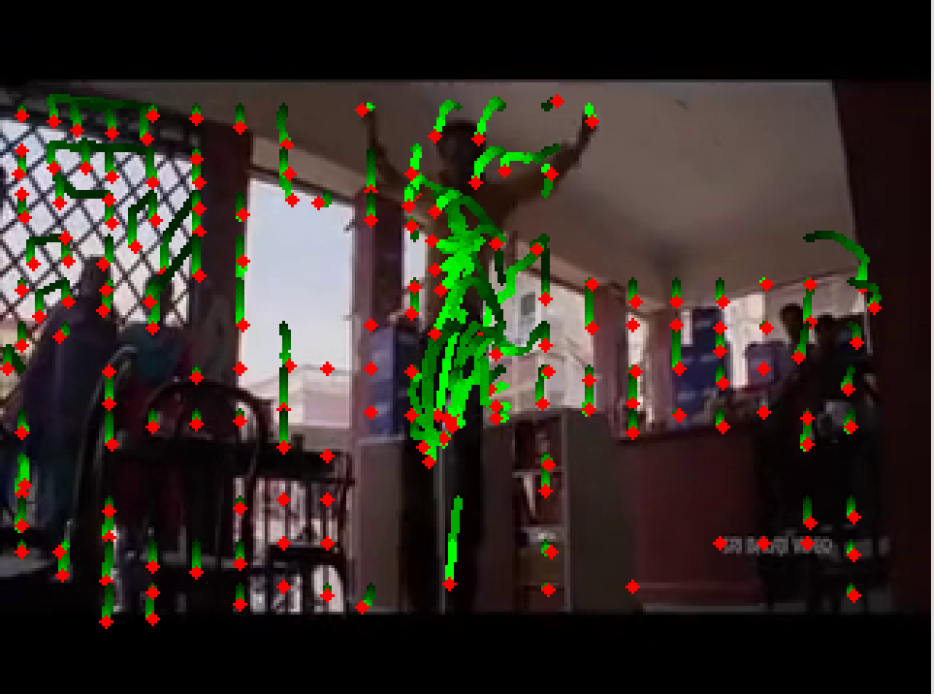
\includegraphics[width=0.6\textwidth]{./images/IDenseTrajVis.png} 
  \caption{A visualization of the improved dense trajectory features for a video
          from the MSR-VTT training set.}
  \label{fig:DenseTrajVis} 
\end{figure*}

Dense trajectory video features have been one of the best-performing features
on various video analysis tasks involving action recognition, despite being
hand-engineered features without any learning from the data.
%%
The technique involves sampling interest points from an initial frame in the
video and tracking these interest points across time.
%%
The location of the interest points which can be tracked reliably are concatenated
to obtain several trajectories in the video.
%%
Local descriptors are then extracted from patches around the points in the
trajectory which serve as features representing the shapes of moving objects.
%%
In this thesis, the same four local descriptors as described
in~\cite{DBLP:conf/cvpr/WangKSL11, Wang2013} are utilized--- namely histogram of
oriented gradients~(HOG), histograms of optical flow~(HOF) and motion boundary
descriptors in horizontal and vertical directions~(MBHx \& MBHy).
%%
Videos can then be represented based on the distribution of the trajectories
they contain.
%%
This can be accomplished by using vector encoding methods such as the bag of
words histogram or Fisher vector encoding~\cite{perronnin2010improving} to
compress the arbitrary number of trajectory features extracted from a video into
a single vector of fixed dimensions.
%%

Both the standard~\cite{DBLP:conf/cvpr/WangKSL11}~(DT) and the improved
versions~\cite{Wang2013}~(IDT) of the dense trajectory features are utilized in
this thesis.
%%
In both versions, the trajectories and their descriptors are first extracted
from the entire video after limiting the trajectories to be a maximum of 15
frames long.
%%
A visualizations of trajectories extracted using the IDT method from a video in
the MSR-VTT training set is shown in Figure~\ref{fig:DenseTrajVis}.
%%
We can see in this example that most of the trajectories are concentrated around
the man performing an action.

Each of the five types of features extracted, trajectory co-ordinates and the
four descriptors, are separately encoded into fixed-size vectors using the
bag-of-features encoding with a codebook of 1000 vectors.
%%
In the bag-of-features encoding, first a fixed codebook containing representative
sample features from the training set is chosen.
%%
In our case, the codebook is obtained using $k$-means clustering on random 250k
trajectory samples from the training set, with $k$=1000.
%%
Then, each feature vector from the set of features of a video is assigned to its
nearest codebook vector.
%%
These assignment counts are accumulated for each codebook entry to give us a
histogram for each video, with the histogram having 1000 bins.
%%
Finally, concatenating the vector encodings of each of the descriptors we get a
video feature vector of 5000 dimensions. 

\subsubsection{3D Convolutional Network}
%%----------------------------------%%
As an alternative to the hand crafted dense trajectory features, video-segment
features are extracted using a deep neural network based on 3-D convolutions. 
%%
Specifically, the C3D~\cite{DBLP:C3D} network, pre-trained on the Sports-1M
dataset, is used.
%%

Inspired by the success of deep 2-D convolutional neural networks as image
feature extractors, the C3D model attempts to employ similar deep networks to learn
video representations.
%%
Since videos have an additional temporal dimension, the 2-D convolutions
used in image CNNs are replaced with 3-dimensional convolutional filters in C3D.
%%
Influenced by the use of small $3\times3$ kernels in the VGG~\cite{Simonyan14c}
network, C3D uses only $3\times3\times3$ convolutional filters.
%%
To prevent too quick loss of temporal information quickly, the pooling
operations are also kept to small windows of size $2\times2\times2$.
%%

The C3D network used in this thesis is pre-trained on the large Sports-1M
dataset, for the task of classifying the video into one among 487 classes of
sports-related actions.
%%
To extract features using C3D, the input videos are first cut into non-overlapping
video segments of 16 frames long.
%%
Then each segment is input into the C3D network and the activations from the
\emph{fc6} and \emph{fc7} layer of the network are extracted as the segment-level
features.
%%
This results in a set of 4096-dimensional feature vectors which represent the
input video and are input to the language model after pooling.

% Comment: If your sentence ends in a capital letter, like here, you should
% write \@ before the period; otherwise LaTeX will assume that this is not
% really an end of the sentence and will not put a large enough space after the
% period. That is, LaTeX assumes that you are (for example), enumerating using
% capital roman numerals, like I. do something, II. do something else. In this
% case, the periods do not end the sentence.

% Similarly, if you do need a normal space after a period (instead of
% the longer sentence separator), use \  (backslash and space) after the
% period. Like so: a.\ first item, b.\ second item.

